\documentclass{article}
\usepackage[utf8]{inputenc}

\usepackage{amsmath}
\usepackage{amssymb}
\usepackage{amsthm}
\usepackage{amsfonts}
\usepackage{graphicx}
\usepackage{multirow}
\usepackage{xcolor}
\usepackage{hyperref}

% For subfigures
\usepackage{subcaption}

\newtheorem{theorem}{Theorem}
\newtheorem{lemma}{Lemma}
\newtheorem{assumption}{Assumption}
\newtheorem{corollary}{Corollary}

\usepackage{natbib}
\usepackage{adjustbox}
\usepackage{tikz}
\usetikzlibrary{shapes, arrows, positioning}

% Remarks by Joni
\usepackage{xcolor}
\newcommand\joni[1]{{\color{red}{{#1}}}}

% \usepackage{authblk}
\title{Possible idea for Vida's paper \#3}



\date{}

\begin{document}

\maketitle

\section{Recap: Univariate time series}

\subsection{Ljung-Box test}

Let $X_t$ be a centered stationary univariate time series process. Consider the null hypothesis

\begin{align*}
    \mathrm{H_{0}}: \mbox{the process $X_t$ is i.i.d.} 
\end{align*}
which says that the time series is essentially noise which does not exhibit any temporal dependence. To test for $H_{0}$, we use the autocorrelations of $X_t$. The lag-$k$ autocorrelation of $X_t$ is defined as $\rho_k = \mathrm{E}(X_t X_{t + k})/\mathrm{E}(X_t^2)$ and measures how strongly correlated each observation is with the one $k$ time steps apart. Given an observed time series $x_1, \ldots, x_T$, the classical Ljung-Box (L-B) test uses for testing $H_0$ the test statistic
\begin{align*}
    \hat{q}_K := T(T + 2) \sum_{k = 1}^K \frac{1}{T - k} \hat{\rho}_k^2,
\end{align*}
where $\hat{\rho}_k$ is the sample lag-$k$ autocorrelation defined as
\begin{align*}
    \hat{\rho}_k = \frac{\frac{1}{T - k} \sum_{t = 1}^{T - k} x_{t} x_{t + k} }{\frac{1}{T} \sum_{t = 1}^{T} x_{t}^2}.
\end{align*}
In case $x_t$ is not a centered process, then the sample time series must be centered by subtracting $\bar{x}$ before the computation of $\hat{\rho}_k$. Under $H_{0}$, we expect each of the $\hat{\rho}_1^2, \ldots, \hat{\rho}_K^2$ to be close to zero and the limiting distribution of $\hat{q}_K$ can be shown to be $\chi^2_K$, meaning that a $p$-value can be obtained as
\begin{align*}
    \mathrm{P}(\chi^2_K > \hat{q}_K).
\end{align*}

\subsection{Autocorrelation function plot}

A visual way of investigating autocorrelations is to plot the pairs $(k, \hat{\rho}_k)$ for $k = 1, \ldots, K$ to produce the so-called autocorrelation function (ACF) plot. This plot can be combined with inferential results by noting that, under $H_{0}$, the limiting distribution of each $\sqrt{T}\hat{\rho}_k$ is $\mathcal{N}(0, 1)$. Hence, by drawing to the ACF plot  horizontal lines at, e.g., heights $\pm 1.96/\sqrt{T} $ lets us visually evaluate whether the observed autocorrelations are significant or not.

\section{New idea: Serial dependence testing for object time series}

\subsection{Metric Ljung-Box test}

Let $(\mathcal{X}, d)$ be a metric space and let $X_t$ be a stationary time series process in $\mathcal{X}$. Our objective is to test the null hypothesis
\begin{align*}
    \mathrm{H_{0}}: \mbox{the process $X_t$ is i.i.d.} 
\end{align*}
Given now an observed object time series $x_1, \ldots, x_T$, we first construct the \textit{metric lag-$k$ autocorrelations}
{\large
\begin{align*}
    \hat{r}_k :=& \frac{\frac{1}{T - k} \sum_{t = 1}^{T - k} \left\{ \frac{1}{\binom{T}{2}} \sum_{i < j} d^2(x_i, x_j) -  d^2(x_t, x_{t + k}) \right\}}{\frac{1}{\binom{T}{2}} \sum_{i < j} d^2(x_i, x_j)} \\
    =& 1 - \frac{\frac{1}{T - k} \sum_{t = 1}^{T - k} d^2(x_t, x_{t + k})}{\frac{1}{\binom{T}{2}} \sum_{i < j} d^2(x_i, x_j)}.
\end{align*}
}
To interpret $\hat{r}_k$, note that $\frac{1}{\binom{T}{2}} \sum_{i < j} d^2(x_i, x_j)$ measures the average squared distance between two elements of the time series. As such, the numerator in the first expression for $\hat{r}_k$ essentially compares whether the squared distances after lag-$k$ jumps deviate from the average squared distance. If $\hat{r}_k > 0$, then after $k$ steps the process is closer to where it started than could be expected from a pure noise process (positive metric autocorrelation), whereas if $\hat{r}_k < 0$, then $k$ steps bring the process further away than expected from noise (negative metric autocorrelation).

To now test for $H_0$, we can use the L-B test statistic
\begin{align*}
    \hat{\ell}_K := T(T + 2) \sum_{k = 1}^K \frac{1}{T - k} \hat{r}_k^2.
\end{align*}
To approximate its null distribution we probably have to resort to a permutation test: shuffle the data arbitrarily to create a time series that has no temporal correlation and use those to compute the null distribution $\hat{\ell}^*_{K, 1}, \ldots, \hat{\ell}^*_{K, B}$.


\begin{center}
    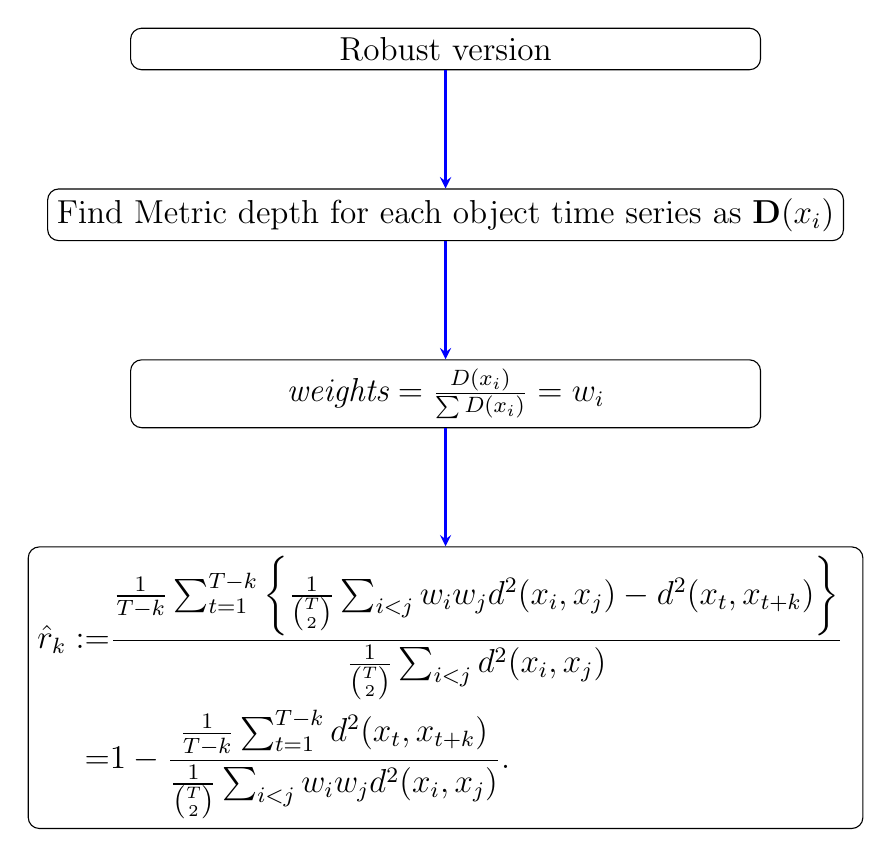
\begin{tikzpicture}[
        node distance=1.5cm and 2cm,
        every node/.style={draw, rounded corners, align=center, minimum width=8cm, font=\large},
        arrow/.style={thick,->,>=stealth, blue}
    ]

    % Nodes
    \node (first) {Robust version};
    \node (start) [below=of first] {Find Metric depth for each object time series as $\mathbf{D}(x_i)$};
    \node (weights) [below=of start] {$\textit{weights} = \frac{D(x_i)}{\sum D(x_i)} = w_i$};
    \node (model) [below=of weights] {
     
     $\begin{aligned}
    \hat{r}_k :=& \frac{\frac{1}{T - k} \sum_{t = 1}^{T - k} \left\{ \frac{1}{\binom{T}{2}} \sum_{i < j} w_iw_jd^2(x_i, x_j) -  d^2(x_t, x_{t + k}) \right\}}{\frac{1}{\binom{T}{2}} \sum_{i < j} d^2(x_i, x_j)} \\
    =& 1 - \frac{\frac{1}{T - k} \sum_{t = 1}^{T - k} d^2(x_t, x_{t + k})}{\frac{1}{\binom{T}{2}} \sum_{i < j} w_iw_jd^2(x_i, x_j)}.
\end{aligned}$
 
    };

    % Arrows
    \draw [arrow] (first) -- (start);
    \draw [arrow] (start) -- (weights);
    \draw [arrow] (weights) -- (model);

    \end{tikzpicture}
\end{center}




\subsection{Metric autocorrelation function plot}

The metric ACF plot can be created analogously, and to obtain the horizontal cut-offs, permutation testing is again needed, separately for each lag $k = 1, \ldots, K$.

\section{Existing literature}

A list of some existing literature about the topic:

\begin{itemize}
    \item \url{https://www.sciencedirect.com/science/article/pii/S0304407623000209} Autoregressive time series for objects living on spheres. No autocorrelation testing is considered.
    \item \url{https://www.tandfonline.com/doi/full/10.1080/01621459.2021.1917416#abstract} Fr{\'e}chet mean trajectories for object time series. No autocorrelation testing is considered.
    \item \url{https://academic.oup.com/jrsssb/article/82/2/275/7056111?guestAccessKey=} Principal component analysis for functional object data, they define a metric autocovariance function that appears to be different from ours. No autocorrelation testing is considered.
    \item \url{https://arxiv.org/abs/2405.03778} Autoregressive model for objects living in a Hadamard space. In Theorem 5.1 they test for lag-1 dependence using the autocovariance test statistic $\frac{1}{T - 1} \sum_{t = 1}^{T - 1} d^2(x_t, x_{t + 1})$. Our proposal can be seen as an improved version of this, in that we allow for multiple lags, we do not restrict to Hadamard spaces and we consider autocorrelation and not autocovariance. This is a possible competitor.
    \item \url{https://academic.oup.com/biomet/article/111/3/925/7413165} They define autodistance covariance for testing serial dependence in object time series. This is a possible competitor.
    \item \url{https://arxiv.org/abs/2506.22361} A general test for independence in object time series. Based on a U-statistic with arbitrary kernel. Maybe too complicated to actually implement as a competitor.
\end{itemize}


% \bibliographystyle{chicago}
% \bibliography{references}



\end{document}

